\section{Motivation} \label{sec:motivation}
Clock frequency determines the accelerator operation speed 
and directly affects the performance. Accordingly, it also has influence on the 
neural network runtime and energy efficiency. In this section, we take 
an open-sourced CNN accelerator named PipeCNN \cite{pipecnn_2} as an example and analyze its 
influence on the neural network performance and energy efficiency.

The accelerator is implemented on KCU1500 and attached to a desktop computer with 
Intel i7-6700@3.40GHz. The basic convolution structure is shown in Fig \ref{fig:cnn-arch}. The largest computing 
array that can be accommodated by the FPGA device consists of 16 dot production units. 
Each dot production unit allows parallel processing of two 8-data vectors.
The accelerator consumes over 11\% LUT of the FPGA device. The optimized clock frequency 
according to the SDAccel compilation is 200 MHz. 

\begin{figure}
	\center{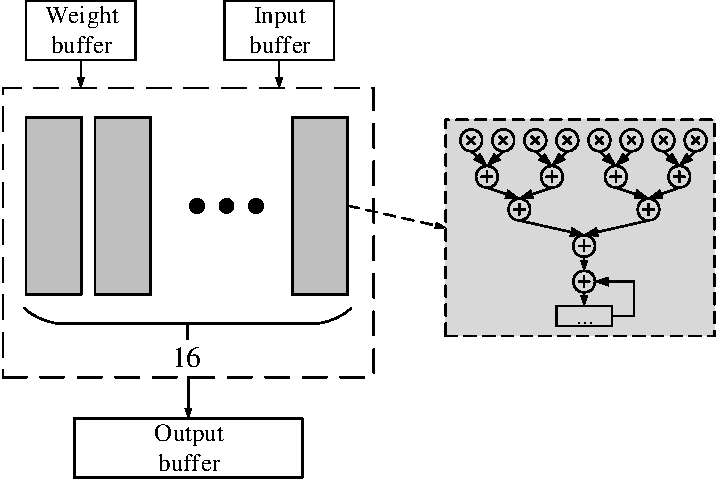
\includegraphics[width=0.75\linewidth]{accelerator}}
    \caption{Baseline CNN accelerator architecture.}
\label{fig:cnn-arch}
\vspace{-1em}
\end{figure}


In order to evaluate the influence of clock 
frequency, we further set the clock to 50 MHz, 100 MHz, and 150 MHz respectively.
A set of neural networks including LeNet, AlexNet, VGG-16 and VGG-19 are used as the benchmark.
Normalized performance the neural network benchmark executed on the accelerators are 
shown in Fig \ref{fig:computing-bound}. It can be found that the 
overall performance of the neural network benchmark
almost increases proportional to the clock frequency. For the larger neural networks, 
the processing remains the computing bound and high frequency design is highly demanded.

\begin{figure}
	\center{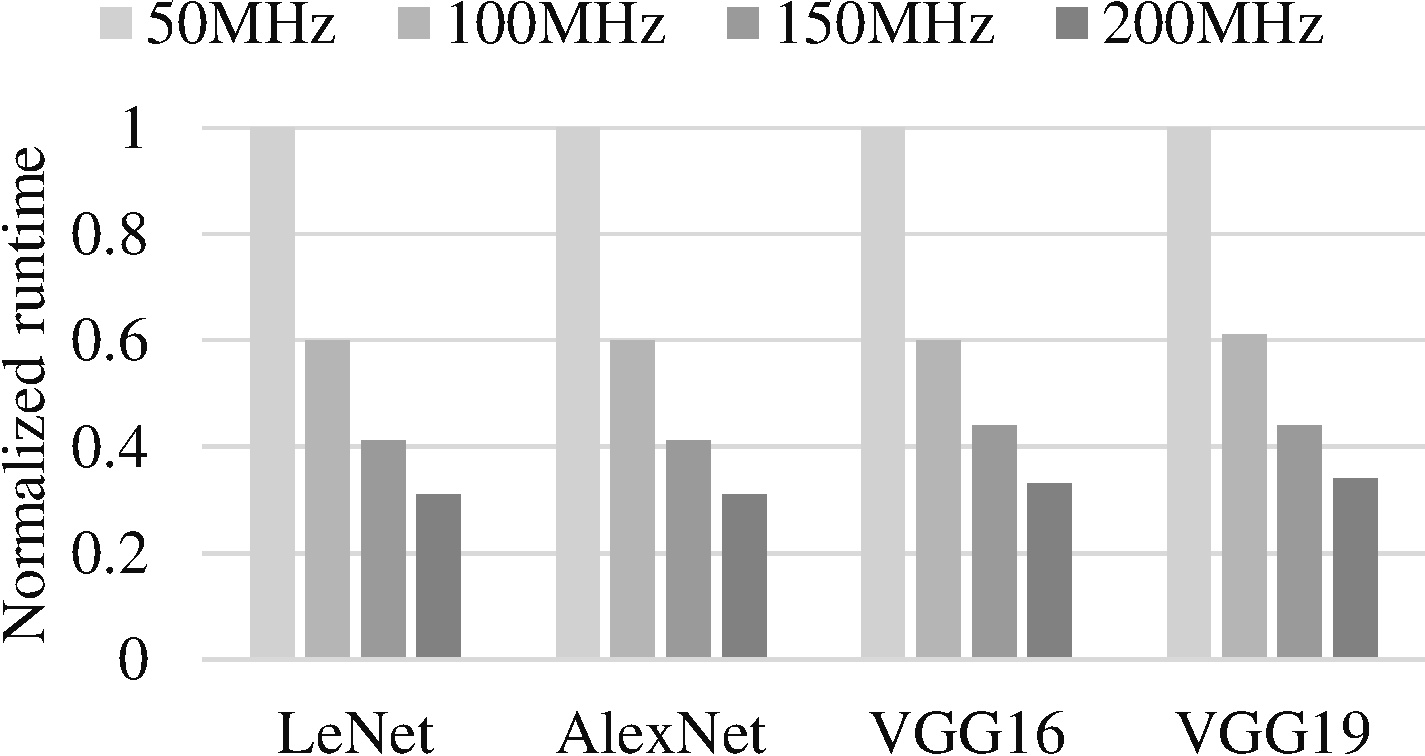
\includegraphics[width=0.75\linewidth]{relative_time}}
    \caption{Normalized performance of neural networks executed on CNN accelerators with different clock frequency.}
\label{fig:computing-bound}
\vspace{-1em}
\end{figure}

In addition, we also obtain the power consumption from SDAccel report. 
The power estimation setup assumes xxxx. Given the power consumption and the performance, 
we calcualted the energy delay product which can be used as an energy efficiency metric.
The energy efficiency is presented in Fig \ref{fig:edp}.
\begin{figure}
	\center{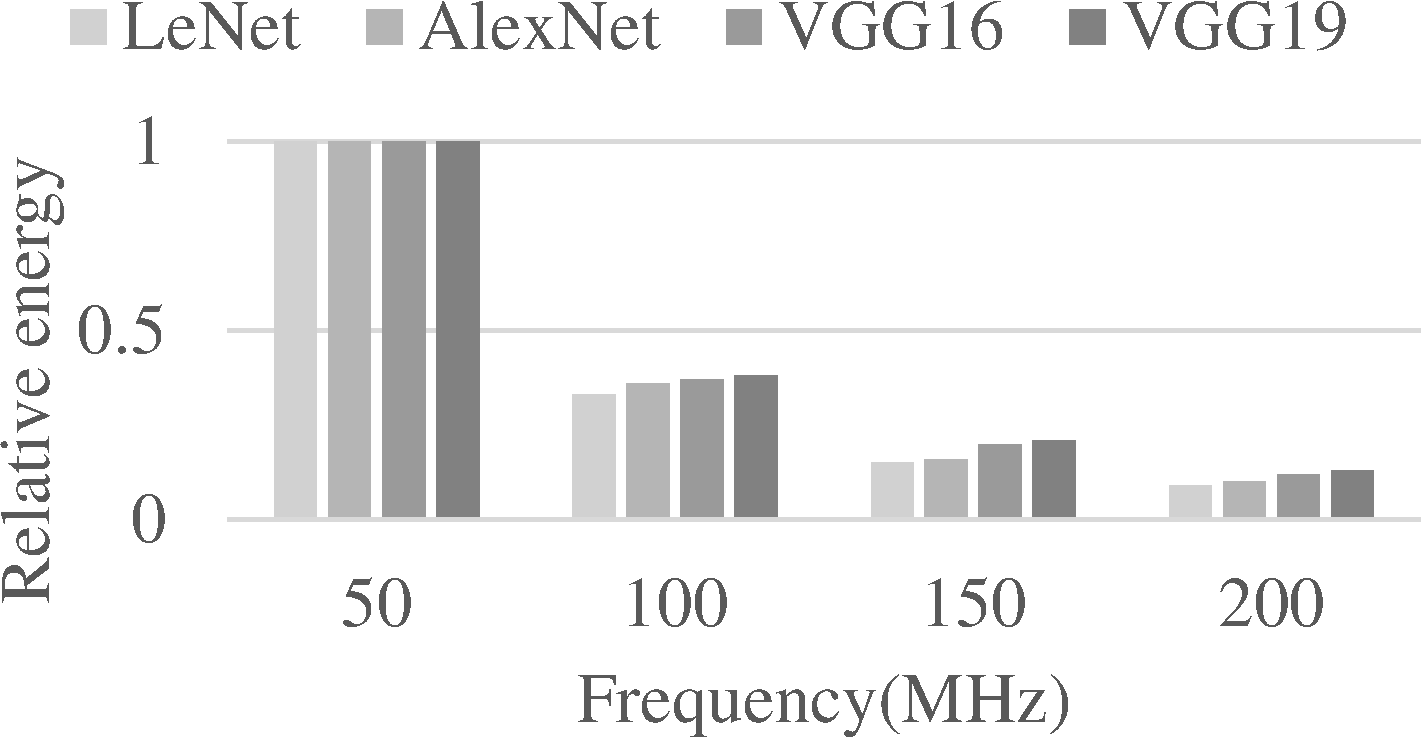
\includegraphics[width=0.75\linewidth]{relative_energy}}
    \caption{Normalized energy-delay product of neural networks executed on CNN accelerators with different clock frequency.}
\label{fig:edp}
\vspace{-1em}
\end{figure}

According to the above experiments, it can be conclcuded that higher clock frequency 
can be beneficial to both the neural network performance and energy efficiency. The 
potential performance and energy efficiency improvement indicates that it is 
worthwhile to boosting the clock of FPGA based CNN accelerators with some minor 
overhead. Detailed overclocking on CNN accelerators will be investigated in 
detail in the rest part of this paper. 
